\paragraph{Final sample}
In
Figures~\ref{fig:finalsample},~\ref{fig:finalsamplecos}~and~\ref{fig:finalsample2d},
one can see the photon energy and angular distribution of the selected
events, respectively. On the same one-dimensionnal figures
(Figures~\ref{fig:finalsample}~and~\ref{fig:finalsamplecos}), the
\Gls{NCg} true events from \Gls{NEUT} distribution is also overlayed
(note that this is done with the version of \Gls{NEUT} which has a bug
in it which results in smaller cross section). This illustrates the
sensitivity of the selection to such processes. One can see from
Figures~\ref{fig:finalsample}~and~\ref{fig:finalsamplecos} that the
selection is dominated by backgrounds and thus the focus of this
analysis is to set a limit on the \Gls{NCg}.

\begin{figure}[ht]
  \center
  \includegraphics[width=0.8\textwidth,page=12]{images/NCg/Selection.pdf}
  \caption[Photon reconstructed energy after the selection]{Photon
    reconstructed energy after the selection with the \Gls{NEUT}
    (5.3.3) \Gls{NCg} cross section and normal magnet \Gls{MC}
    simulations.}
  \label{fig:finalsample}
\end{figure}

\begin{figure}[ht]
  \center
  \includegraphics[width=0.8\textwidth,page=13]{images/NCg/Selection.pdf}
  \caption[Photon reconstructed $\cos(\theta)$ after the
  selection]{Photon reconstructed $\cos(\theta)$ after the selection
    with the \Gls{NEUT} (5.3.3) \Gls{NCg} cross section and normal
    magnet \Gls{MC}.}
  \label{fig:finalsamplecos}
\end{figure}

\begin{figure}[ht]
  \center
  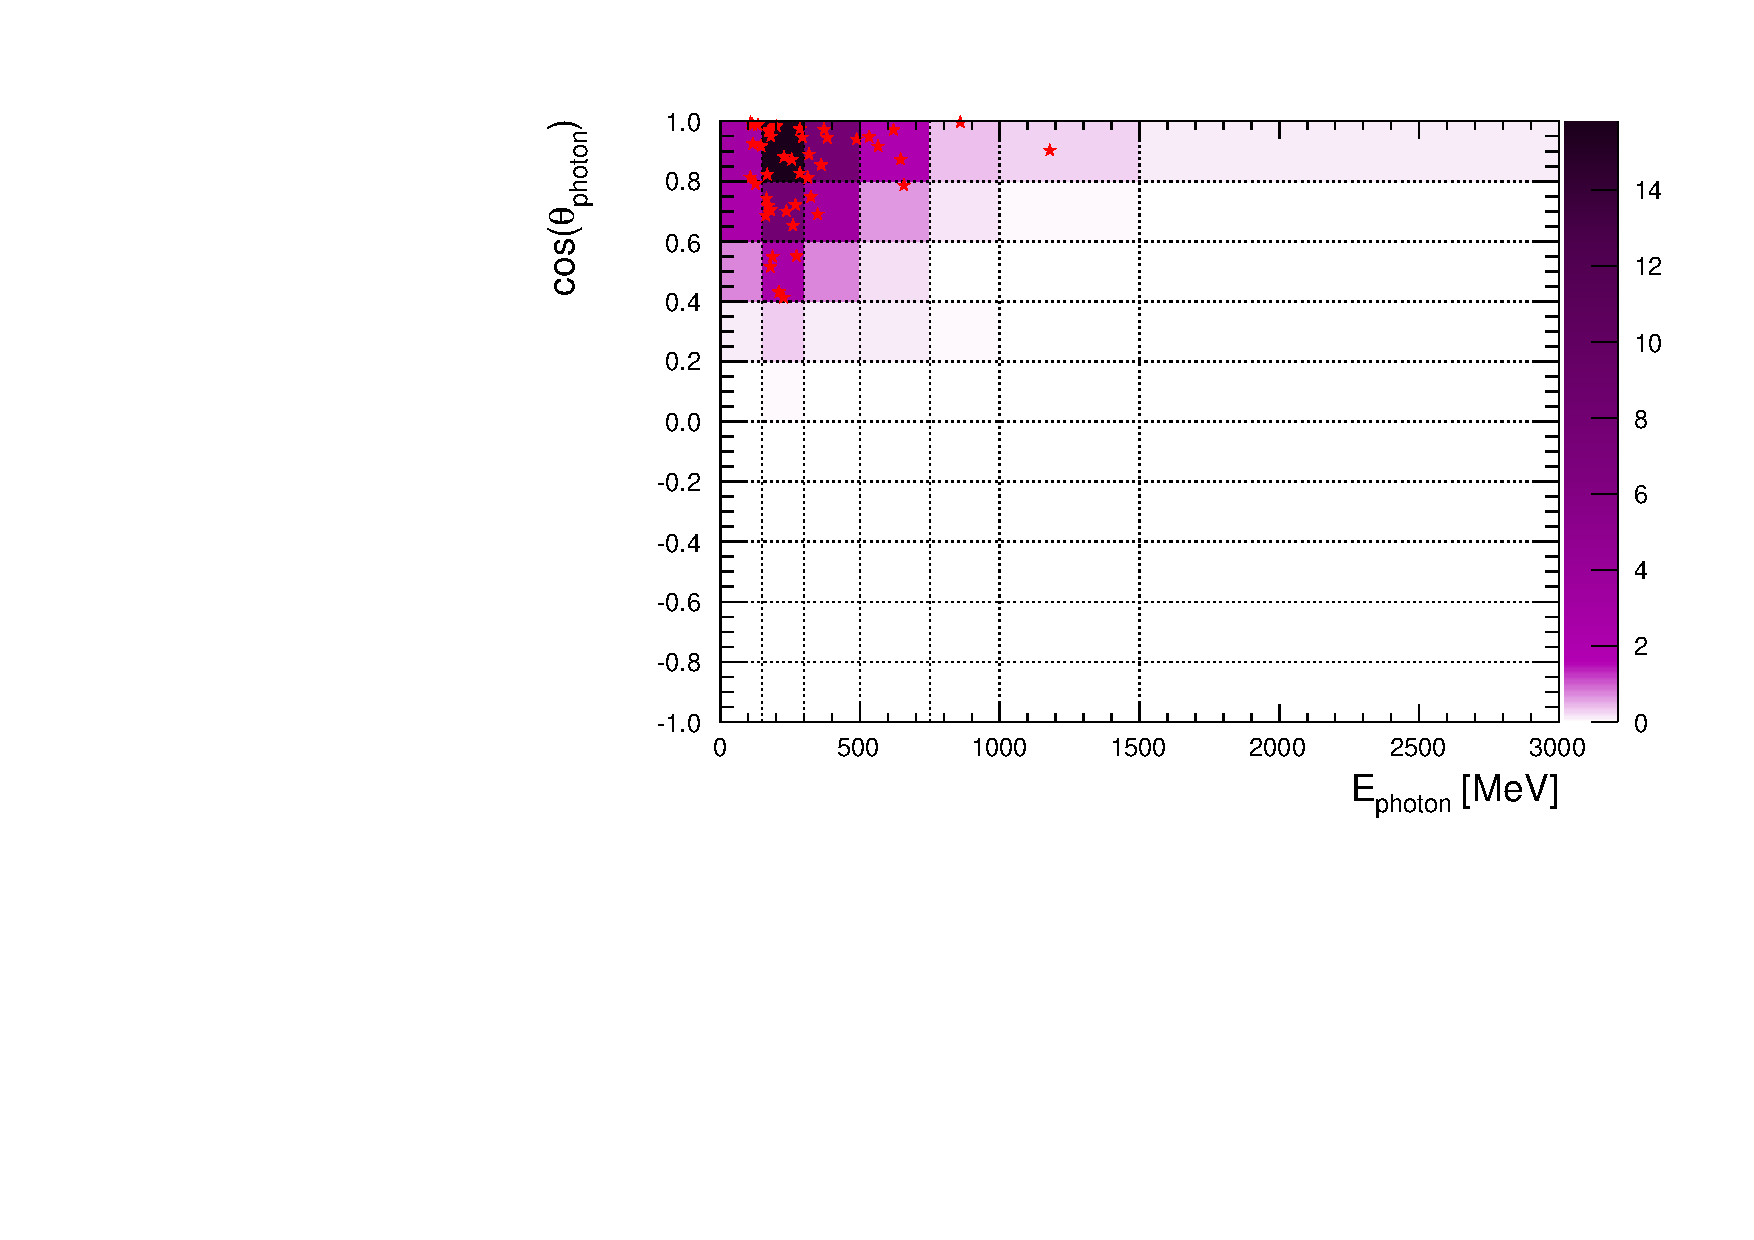
\includegraphics[width=0.8\textwidth]{images/NCg/gamma2D.pdf}
  \caption[Photon reconstructed $\cos(\theta)$ and energy after the
  selection]{Photon reconstructed $\cos(\theta)$ and energy after the
    selection, the stars indicate the data points.}
  \label{fig:finalsample2d}
\end{figure}


To further clarify the content of the selection, breakdowns by target,
reaction and topology are realised in
Tables~\ref{tab:target},~\ref{tab:reaction}~and~\ref{tab:topo},
respectively. Note that the \Gls{FGD}1 external photon events have
been separated from the internal ones. These tables highlight the
difficulties to perform such a measurement: even after essentially
blocking all the upstream activity, the selection still contains
around 35\% of \Gls{OOFV} events. This comes from the dead material
regions which are not instrumented and for which it is not possible to
veto the event. Table~\ref{tab:target} shows the breakdown by target,
from which it can be concluded that most of these events happen on the
support structure (aluminium) or on the case of the \Gls{TPC}
(carbon), or in regions close to the edge of the detector where no
object has been reconstructed (for example, lead events come from the
\Gls{ECal}, but these events do not create any object in the
\Gls{ECal}). The spatial distributions of these events are shown in
Appendix~\ref{app:oofvphoton}.

Similarly, one can see on Table~\ref{tab:reaction} that some \Gls{CC}
events do survive the \Gls{CC} veto; these events probably have a low
momentum muon which makes them go below a number of node threshold to
be identified as muon.

Finally, the Table~\ref{tab:topo} highlights the difficulties to
detect and reconstruct the secondary photon from neutral pion
decay. Most of the time, the photon that creates the
electron~/~positron pair in the \Gls{FGD}1 is the most energetic one,
and, since the neutral pion has a relatively small kinetic energy, the
secondary photon has quite low energy and is not detected.



\begin{table}[ht]
  \begin{adjustbox}{center}
    \begin{tabular}{ccc}
      \toprule
      Target & NEvents & Percentage \\
      \midrule
      carbon          & 32.18 & 55.32 \\
      oxygen          & 1.20  & 2.06  \\
      hydrogen        & 2.36  & 4.05  \\
      other           & 0.88  & 1.51  \\
      \midrule
      Total inside \Gls{FGD}1 \Gls{FV}  & 36.61 &  62.94 \\ 
      \midrule
      carbon          & 8.85  & 15.21 \\
      oxygen          & 1.34  & 2.30  \\
      hydrogen        & 0.49  & 0.84  \\
      aluminium       & 4.79  & 8.24  \\
      iron            & 2.59  & 4.45  \\
      copper          & 0.10  & 0.17  \\
      lead            & 2.57  & 4.41 \\
      other           & 0.84  & 1.45  \\
      \midrule
      Total outside \Gls{FGD}1 \Gls{FV} & 21.56 & 37.06 \\
      \bottomrule
    \end{tabular}
  \end{adjustbox}
  \caption[Neutrino target for the selected events]{Neutrino target
    for the selected events, separated for external photons and for
    \Gls{FGD}1 \Gls{FV} photons}
  \label{tab:target}
\end{table}

\begin{table}[ht]
  \begin{adjustbox}{center}
    \begin{tabular}{ccc}
      \toprule
      Reaction & NEvents & Percentage \\
      \midrule
      \gls{numu} \Gls{CCQE}                    & 0.41 & 0.70  \\
      \gls{numu} \Gls{CC} \Gls{RES} \gls{piz}  & 4.81 & 8.24  \\
      \gls{numu} \Gls{CC} \Gls{RES} \gls{pipm} & 4.18 & 7.16  \\
      \gls{numu} \Gls{CC} \Gls{SIS}~/~\Gls{DIS}& 0.73 & 1.25  \\
      \Gls{NC} \Gls{RES} \gls{piz}             & 11.71& 20.05 \\
      \Gls{NC} \Gls{RES} \gls{pipm}            & 9.63 & 16.49 \\
      \Gls{NC} \Gls{SIS}~/~\Gls{DIS}           & 0.84 & 1.44  \\
      \Gls{NC} single $\gamma$                 & 0.14 & 0.24  \\
      other                                    & 4.30 & 7.36  \\
      \midrule
      Total inside \Gls{FGD}1 \Gls{FV}         & 36.75& 62.94 \\
      \midrule
      \gls{numu} \Gls{CCQE}                    & 1.52 & 2.60  \\
      \gls{numu} \Gls{CC} \Gls{RES} \Gls{piz}  & 2.54 & 4.35  \\
      \gls{numu} \Gls{CC} \Gls{RES} \Gls{pipm} & 2.84 & 4.86  \\
      \gls{numu} \Gls{CC} \Gls{SIS}~/~\Gls{DIS}& 0.61 & 1.04  \\
      \Gls{NC} \Gls{RES} \Gls{piz}             & 5.39 & 9.23  \\
      \Gls{NC} \Gls{RES} \Gls{pipm}            & 5.85 & 10.02 \\
      \Gls{NC} \Gls{SIS}~/~\Gls{DIS}           & 0.86 & 1.47  \\
      \Gls{NC} single $\gamma$                 & 0.10 & 0.17 \\
      other                                    & 1.93 & 3.31  \\
      \midrule
      Total outside \Gls{FGD}1 \Gls{FV}        & 21.56 & 37.06 \\ 
      \bottomrule
    \end{tabular}
  \end{adjustbox}
  \caption[Neutrino true interaction modes for the selected
  events]{Neutrino true interaction modes for the selected events,
    separated for external photons and for \Gls{FGD}1 \Gls{FV}
    photons.  Note that the \Gls{NCg} component was derived with a
    high statistic sample generated independently.}
  \label{tab:reaction}
\end{table}


\begin{table}[ht]
  \begin{adjustbox}{center}
    \begin{tabular}{ccc}
      \toprule
      Topology & NEvents & Percentage \\
      \midrule
      \Gls{numu} \Gls{CC}0$\pi$       & 0.51  & 0.87  \\
      \Gls{numu} \Gls{CC}1\Gls{piz}   & 5.93  & 10.17 \\
      \Gls{numu} \Gls{CC}1\Gls{pipm}  & 1.40  & 2.40  \\
      \Gls{numu} \Gls{CC} multi-$\pi$ & 2.00  & 3.43  \\
      \Gls{NC} 1\Gls{piz}             & 19.50 & 33.44 \\
      \Gls{NC} 1\Gls{pipm}            & 0.35  & 0.60  \\
      \Gls{NC} multi-$\pi$            & 2.02  & 3.46  \\
      \Gls{NC} single $\gamma$        & 0.14  & 0.24  \\
      other                           & 4.89  & 8.38  \\
      \midrule
      Total inside \Gls{FGD}1 \Gls{FV}& 36.75 & 62.94 \\ 
      \midrule
      \Gls{numu} \Gls{CC}0$\pi$       & 1.92  & 3.29  \\
      \Gls{numu} \Gls{CC}1\Gls{piz}   & 3.53  & 6.05  \\
      \Gls{numu} \Gls{CC}1\Gls{pipm}  & 0.68  & 1.17  \\
      \Gls{numu} \Gls{CC} multi-$\pi$ & 0.94  & 1.61  \\
      \Gls{NC} 1\Gls{piz}             & 10.15 & 17.40 \\
      \Gls{NC} 1\Gls{pipm}            & 0.40  & 0.69  \\
      \Gls{NC} multi-$\pi$            & 1.96  & 3.36  \\
      \Gls{NC} single $\gamma$        & 0.10  & 0.17  \\
      other                           & 1.90  & 3.26  \\
      \midrule
      Total outside \Gls{FGD}1 \Gls{FV}& 21.56 & 37.06 \\
      \bottomrule
    \end{tabular}
  \end{adjustbox}
  \caption[Topology of the selected events]{Topology of the selected
    events, separated for external photons and for \Gls{FGD}1 \Gls{FV}
    photons.  Note that the \Gls{NCg} component was derived with a
    high statistic sample generated independently.}
  \label{tab:topo}
\end{table}

Based on the Table~\ref{tab:topo}, and the fact that the analysis is
dominated by backgrounds, it should be concluded that the final result
of this analysis will be a limit on the \Gls{NCg}
processes. Therefore, the uncertainties on the background are the main
drive of the limit.

With this number of events, the statistical uncertainty on the limit
is roughly less than 15~\%. This is already smaller than the expected
error for \Gls{OOFV} events as will be detailed later. It was
concluded that the error on this sample is already largely limited by
systematic errors and therefore it makes sense to conduct this
analysis now.

\clearpage
\paragraph{Efficiencies}

Upon deciding the cut values; one is interested whether the cuts are
actually the best way of selecting the \Gls{NCg} events; the effect of
all the cuts on the efficiency\footnote{The efficiency is defined here
  as the following ratio:
  $\frac{\text{Number of selected NC}\gamma\text{ events}}{\text{Total
      number of NC}\gamma\text{ events generated}}$} to select the
\Gls{NCg} events is shown Figure~\ref{fig:effvscuts}. On this plot,
one notices the relative low impact of the vetoes on the selections
and that one of the largest drop in efficiency comes from requiring
track propagating in the \Gls{TPC}. This is probably because of the
high angle photons that get cut away from the selection (this is also
visible in bottom of Figure~\ref{fig:photoneff1}).

Another concern is the \Gls{PID} cuts: in
Figure~\ref{fig:tpcpullprim}, one sees that all the electrons and
positrons are within the cut lines, so one could wonder why the
efficiency is impacted by these cuts as can be seen in
Figure~\ref{fig:effvscuts}. The reason why this cut removes half of
the events is because the protons coming out of the vertex can
sometimes be the \Gls{MT} or the \Gls{PT}. As can be seen in
Figure~\ref{fig:pullncg}, if the \Gls{PID} cuts were made looser, the
efficiency would become higher after both the \Gls{PID} cut, but the
invariant mass will reject the events, since they have different
kinematics.

Another interesting feature is the \Gls{ECal} veto, which halves the
efficiency. This is because the \Gls{MT} and \Gls{PT} can lose energy
via bremsstrahlung and eventually create an unmatched object in the
\Gls{ECal}, however it is quite complicated to differentiate these
from a secondary photon coming from a \Gls{piz}, so it was chosen to
leave the cut as it is.

\begin{figure}[ht]
  \center
  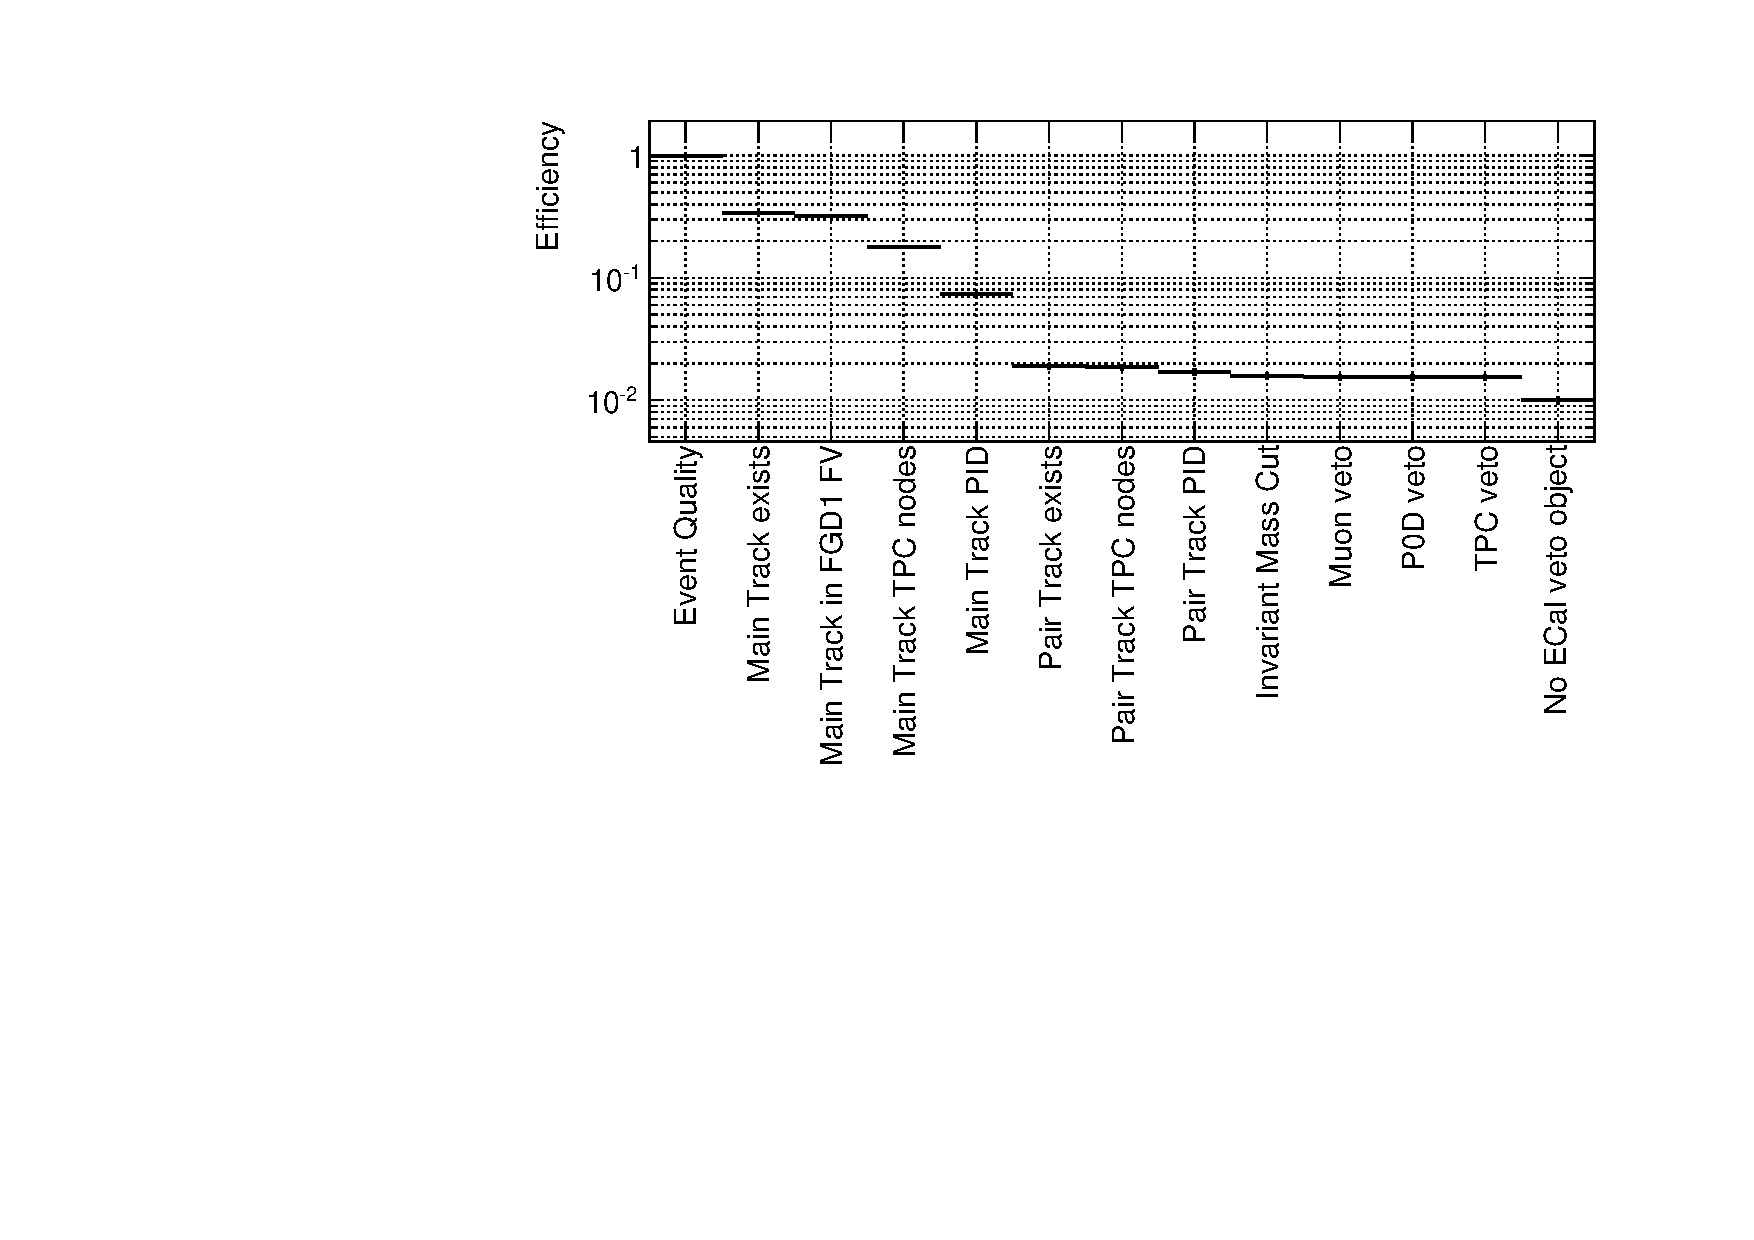
\includegraphics[width=0.8\textwidth]{images/NCg/eff_cut.pdf}
  \caption[NEUT FGD1 NC$\gamma$ efficiency against selection
  cut]{Efficiency against selection cut for \Gls{NEUT} \Gls{NCg}
    events happening in the \Gls{FGD}1 (errors are statistical).}
  \label{fig:effvscuts}
\end{figure}


\begin{figure}[ht]
  \center
  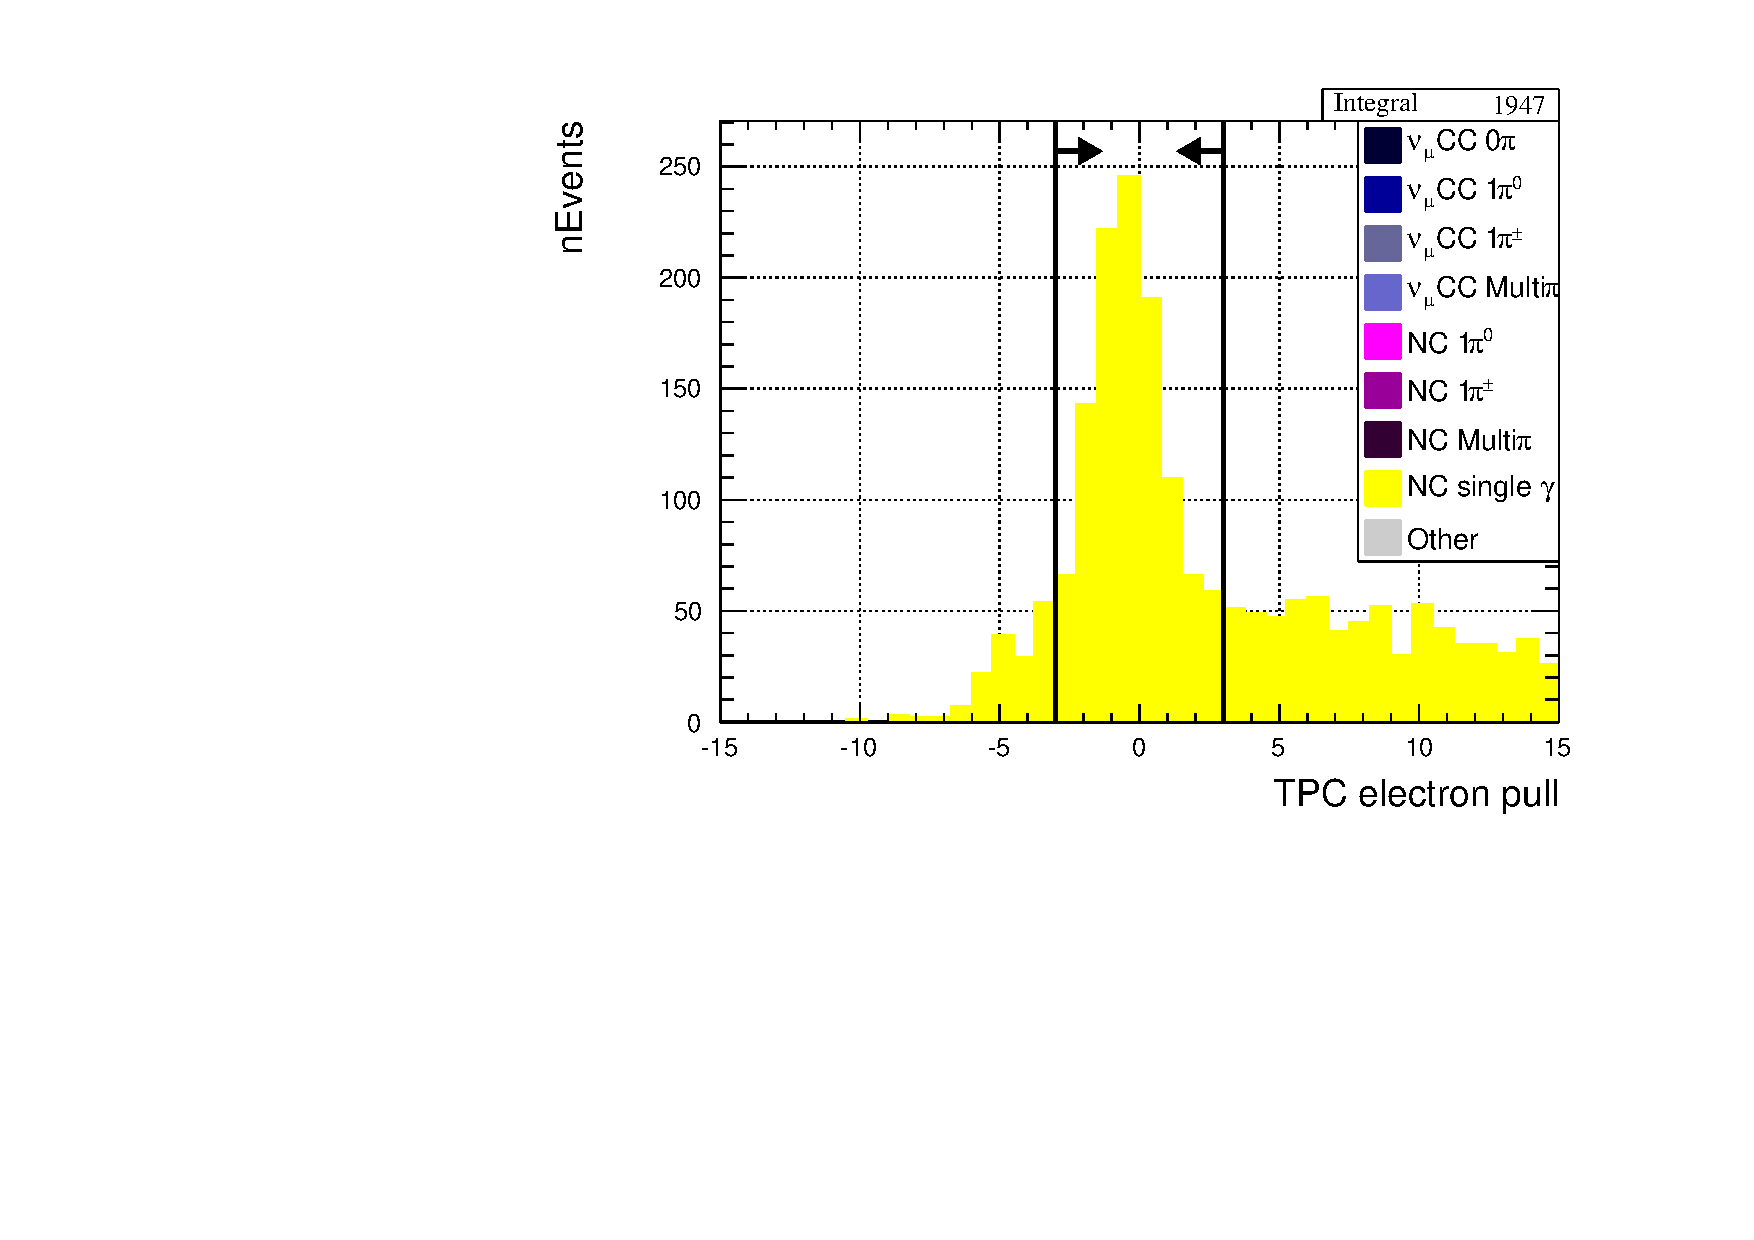
\includegraphics[width=0.8\textwidth]{images/NCg/3_selelec_tpc1_pullelec_pitoponcg.pdf} \\
  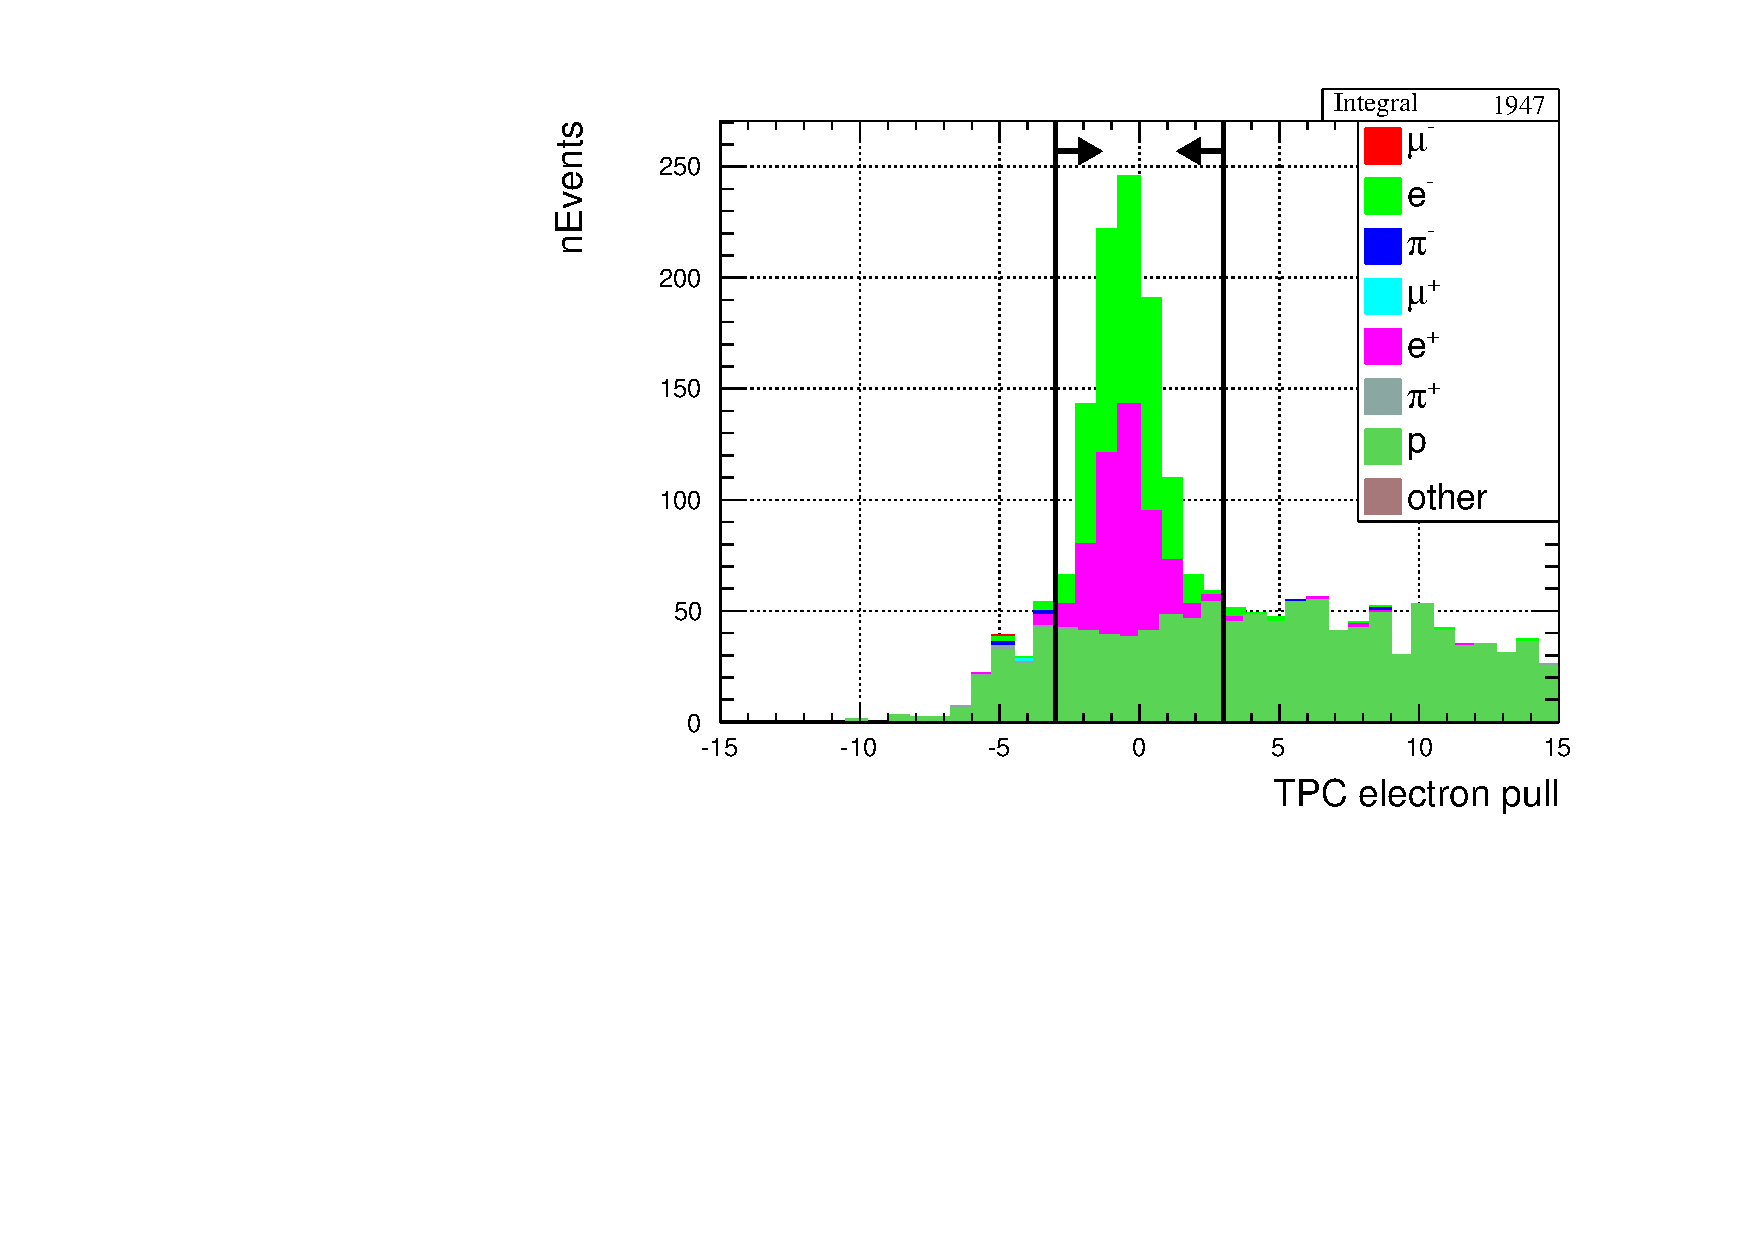
\includegraphics[width=0.8\textwidth]{images/NCg/3_selelec_tpc1_pullelec_particle.pdf}
  \caption[TPC pull cut for Main Track if the interaction was a true
  NC$\gamma$ event happening in the FGD1]{\Gls{TPC} pull cut for
    \Gls{MT} if the interaction was a true \Gls{NCg} event happening
    in the \Gls{FGD}. \textbf{\textit{Top:}} For each interaction
    channel. \textbf{\textit{Bottom:}} For each the particle type.
    All the excluded events are protons. The cut values are depicted
    by the black lines.}
  \label{fig:pullncg}
\end{figure}

Using the selection as described, and the \Gls{NCg} enhanced \Gls{MC},
the one-dimensionnal photon efficiencies were computed for signal and
background photons, as can be seen in Figures~\ref{fig:photoneff1} and
\ref{fig:photoneff2}. Note that a background event for the calculation
of the efficiency is defined as ``any event that creates a photon in
the \Gls{FGD}1 or that creates a photon entering the \Gls{FGD}1''.

\begin{figure}[ht]
  \center
  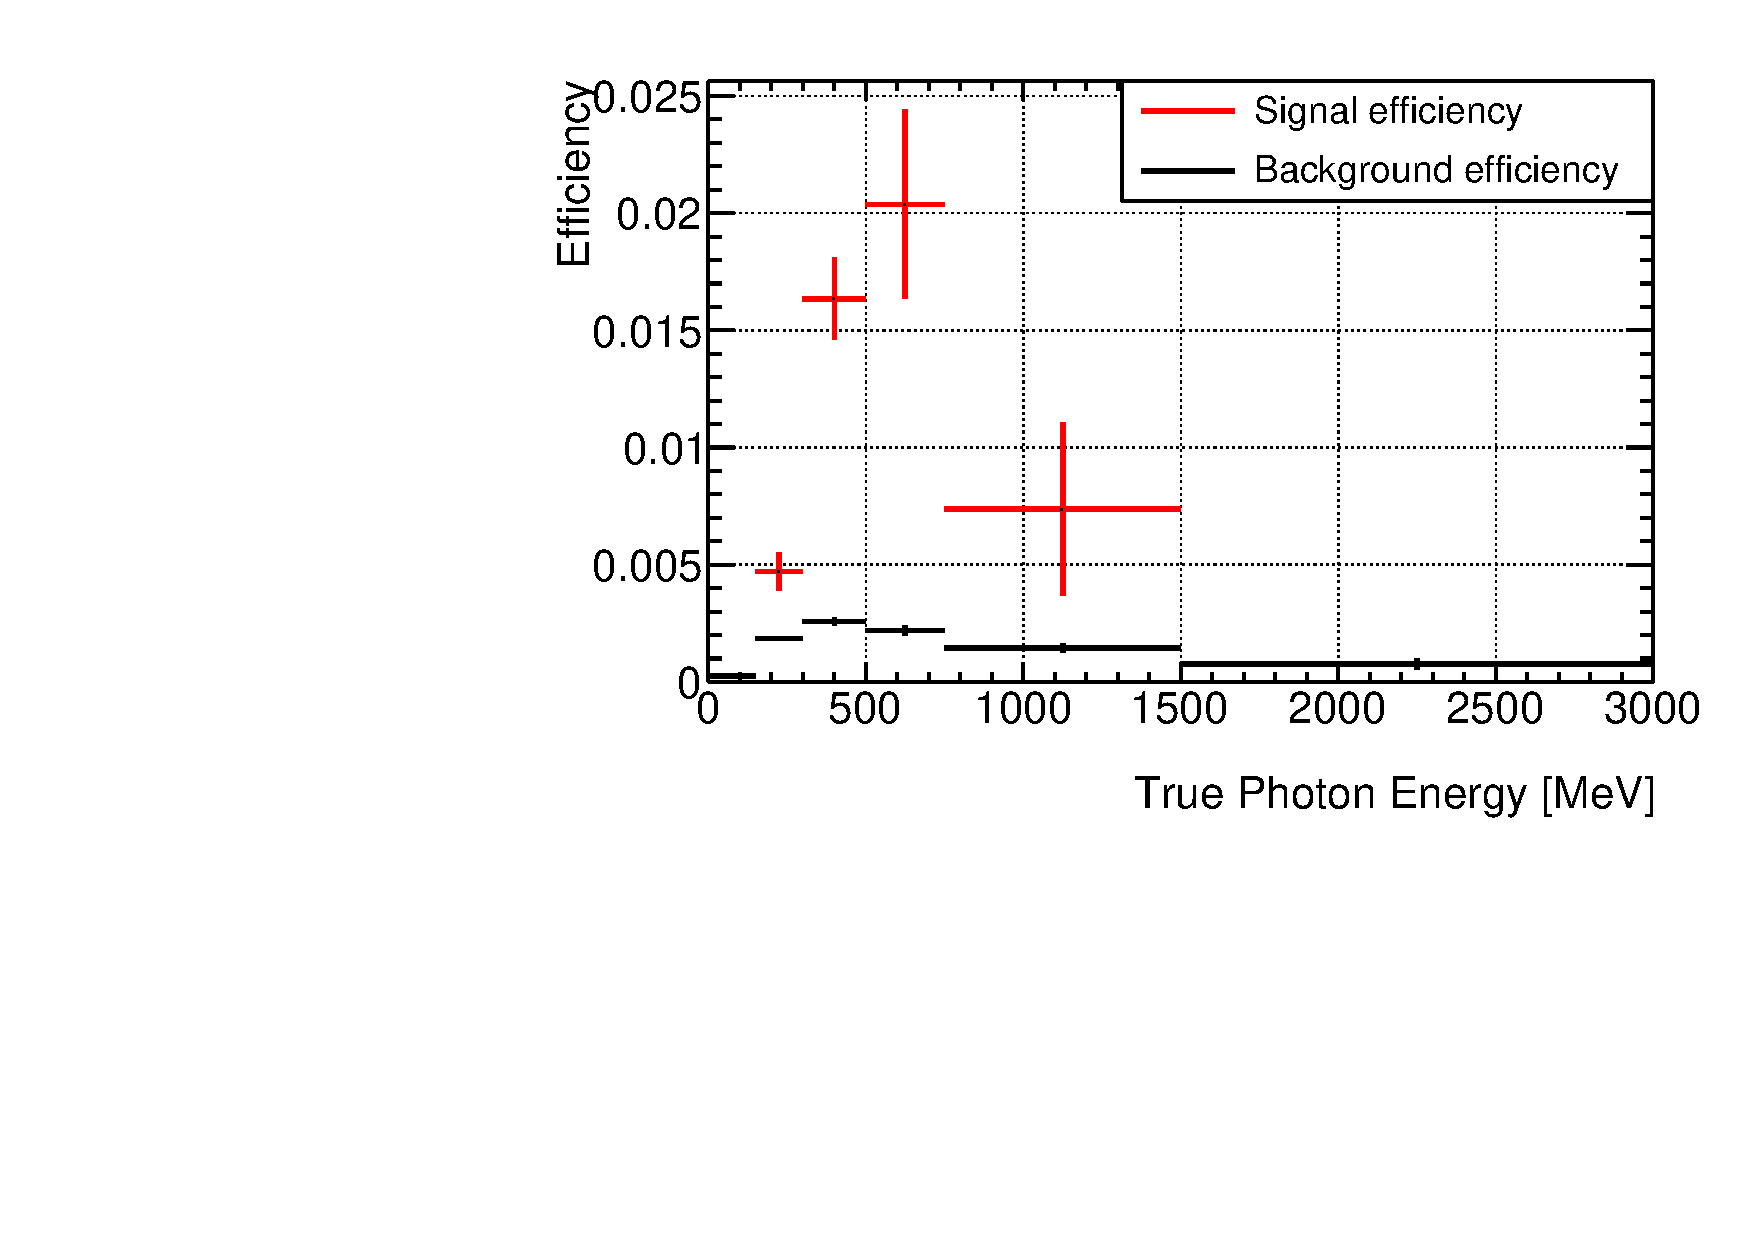
\includegraphics[width=0.8\textwidth]{images/NCg/Eff_gamma_mom.pdf}\\
  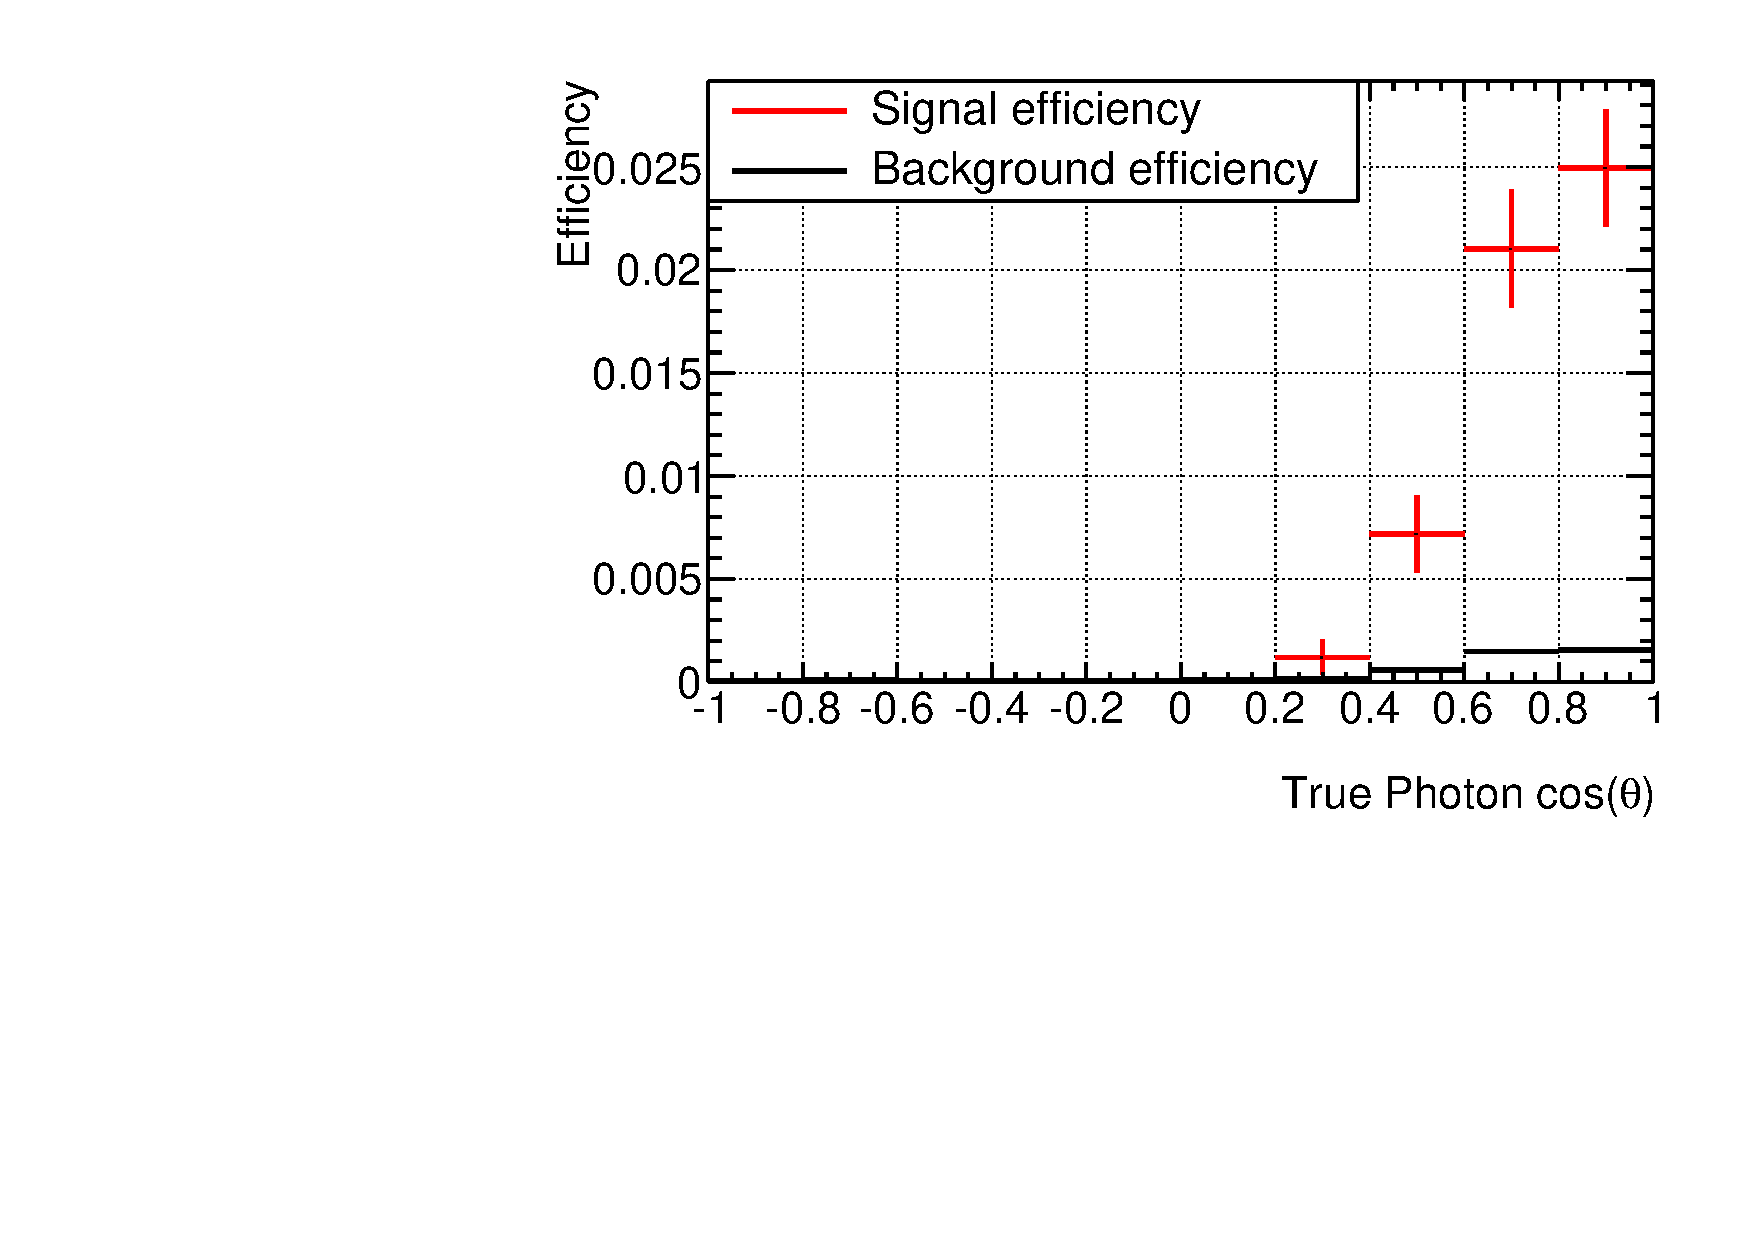
\includegraphics[width=0.8\textwidth]{images/NCg/Eff_gamma_cos.pdf}
  \caption[Photon selection efficiency for signal events and for
  background events against photon energy and photon angle
  ($\cos(\theta)$).]{Photon selection efficiency for signal events and
    for background events (errors are
    statistical. \textbf{\textit{Top:}} Efficiency against the photon
    energy. \textbf{\textit{Bottom:}} Efficiency against the photon
    angle ($\cos(\theta)$).}
  \label{fig:photoneff1}
\end{figure}

\begin{figure}[ht]
  \center
  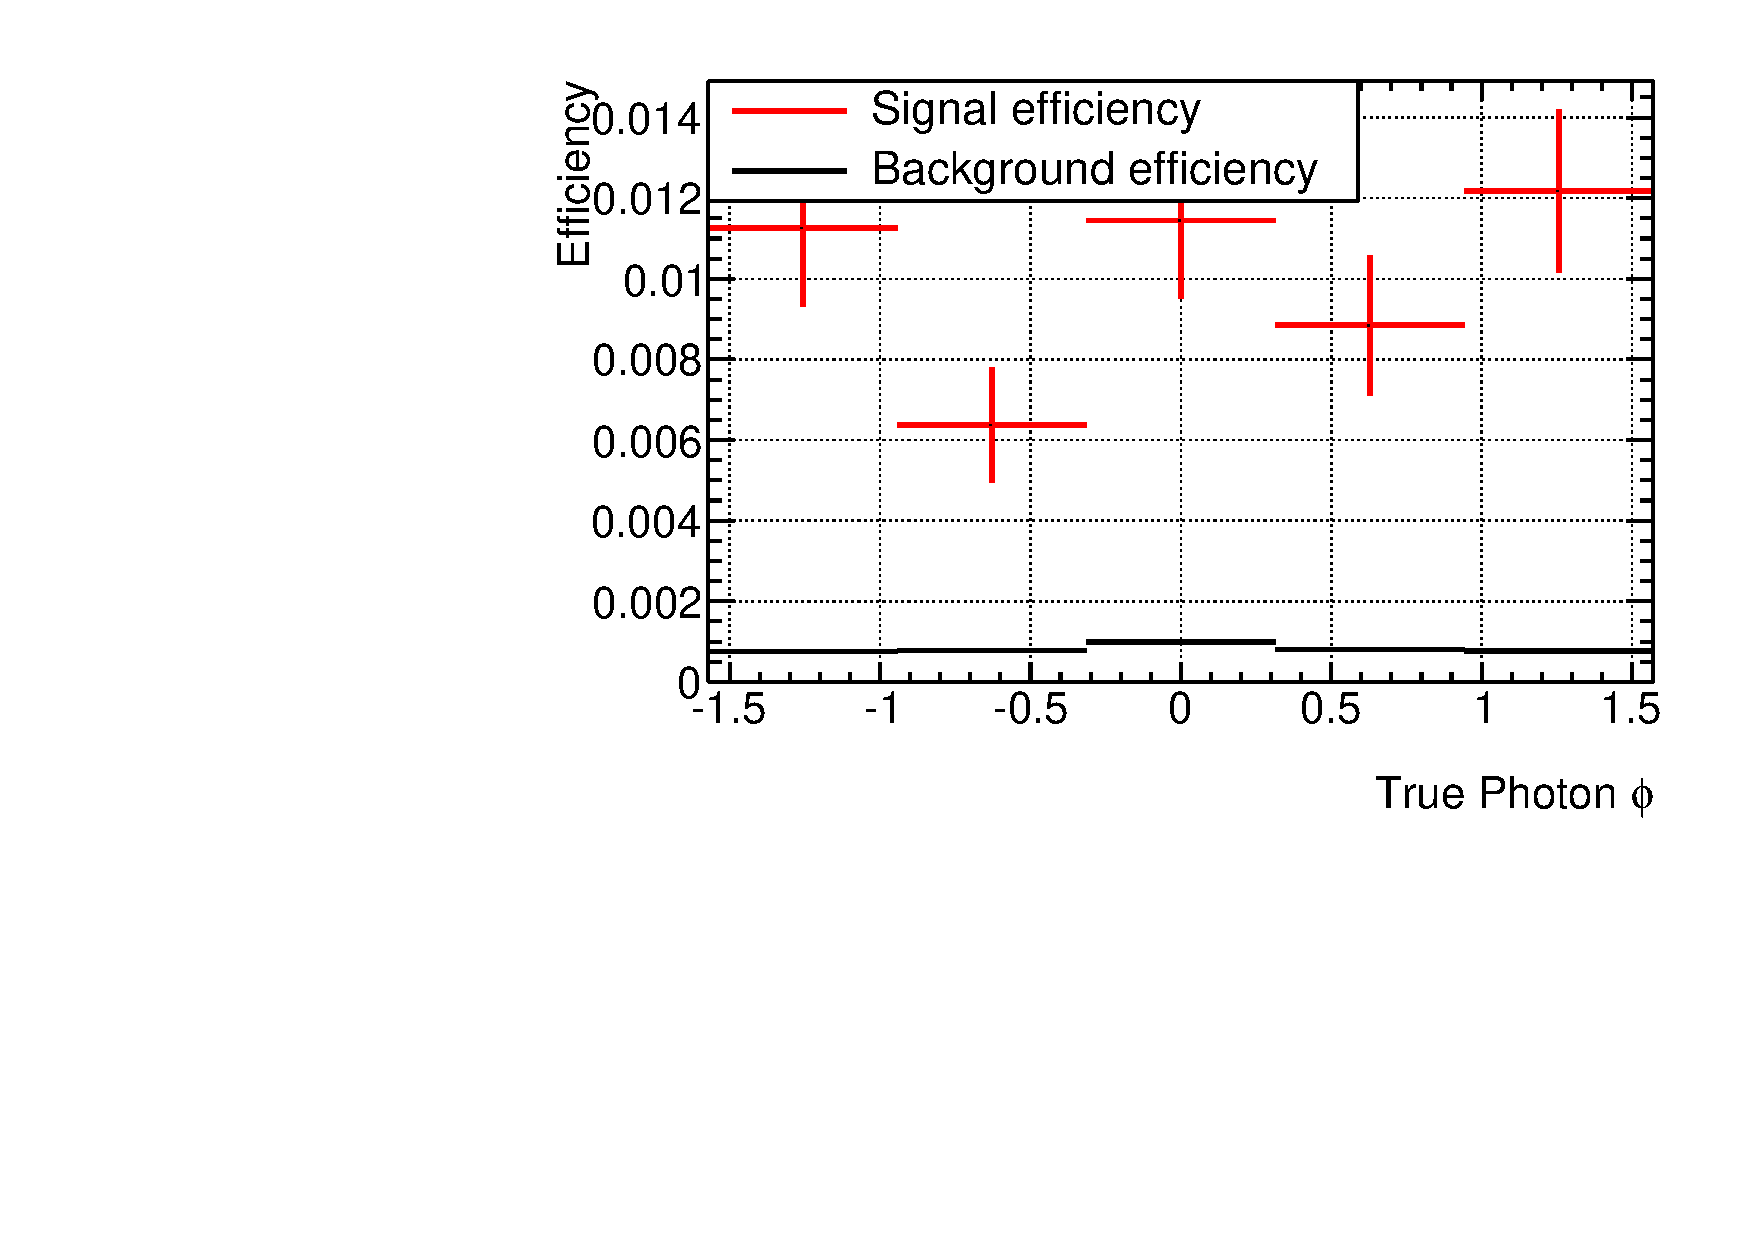
\includegraphics[width=0.8\textwidth]{images/NCg/Eff_gamma_phi.pdf}\\
  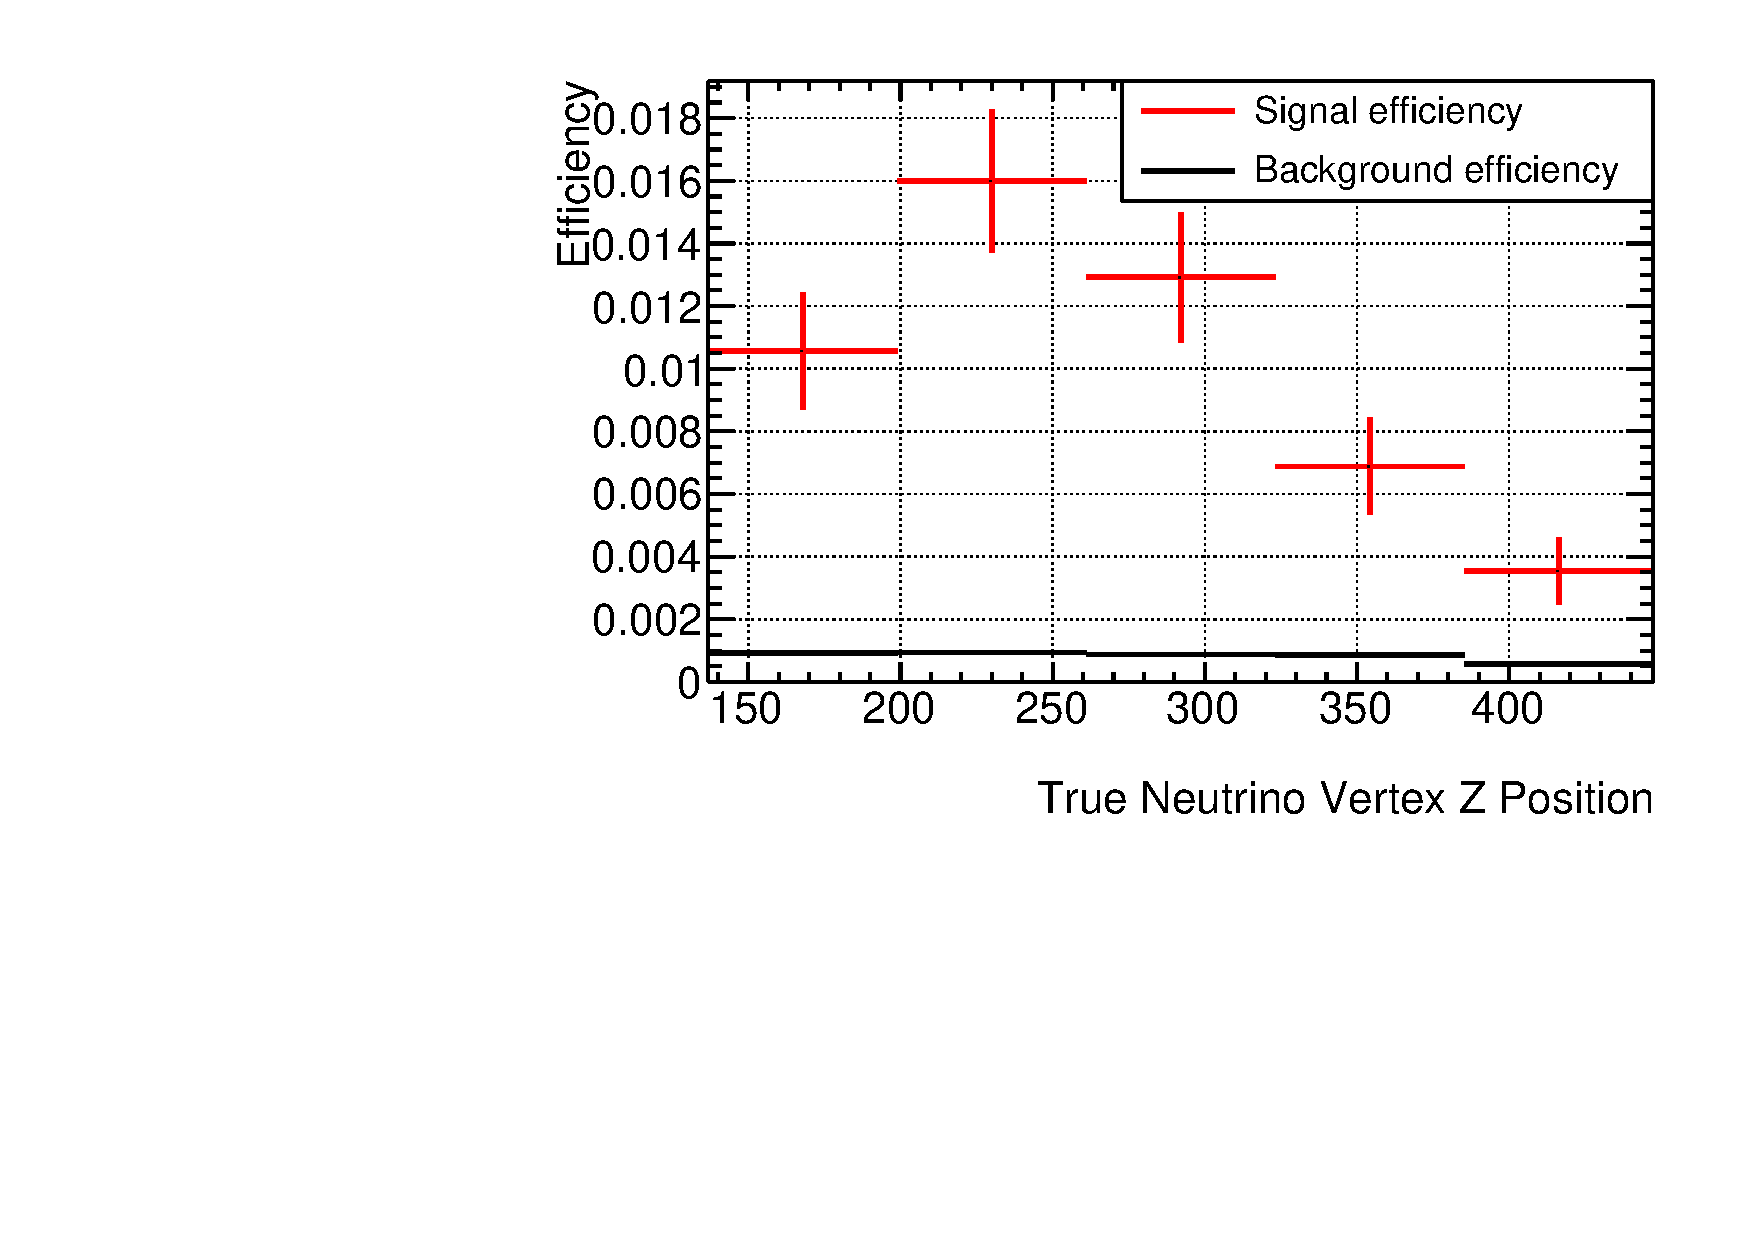
\includegraphics[width=0.8\textwidth]{images/NCg/Eff_gamma_pos.pdf}
  \caption[Photon selection efficiency for signal events and for
  background events against photon azimuthal angle and photon creation
  point.]{Photon selection efficiency for signal events and for
    background events (errors are statistical). \textbf{\textit{Top:}}
    Efficiency against the photon azimuthal
    angle. \textbf{\textit{Bottom:}} Efficiency against the photon Z
    starting point in the \Gls{FGD}1.}
  \label{fig:photoneff2}
\end{figure}

Similarly, since the \Gls{piz} are the major background of the
analysis, the efficiency of the different processes creating \Gls{piz}
in terms of the \Gls{piz} kinematics in Figures~\ref{fig:pizeff1} and
\ref{fig:pizeff2} were calculated. In this case, this is shown before
and after the vetoes, since they are expected to have a significant
effect on the \Gls{piz} efficiency.

\begin{figure}[ht]
  \center
  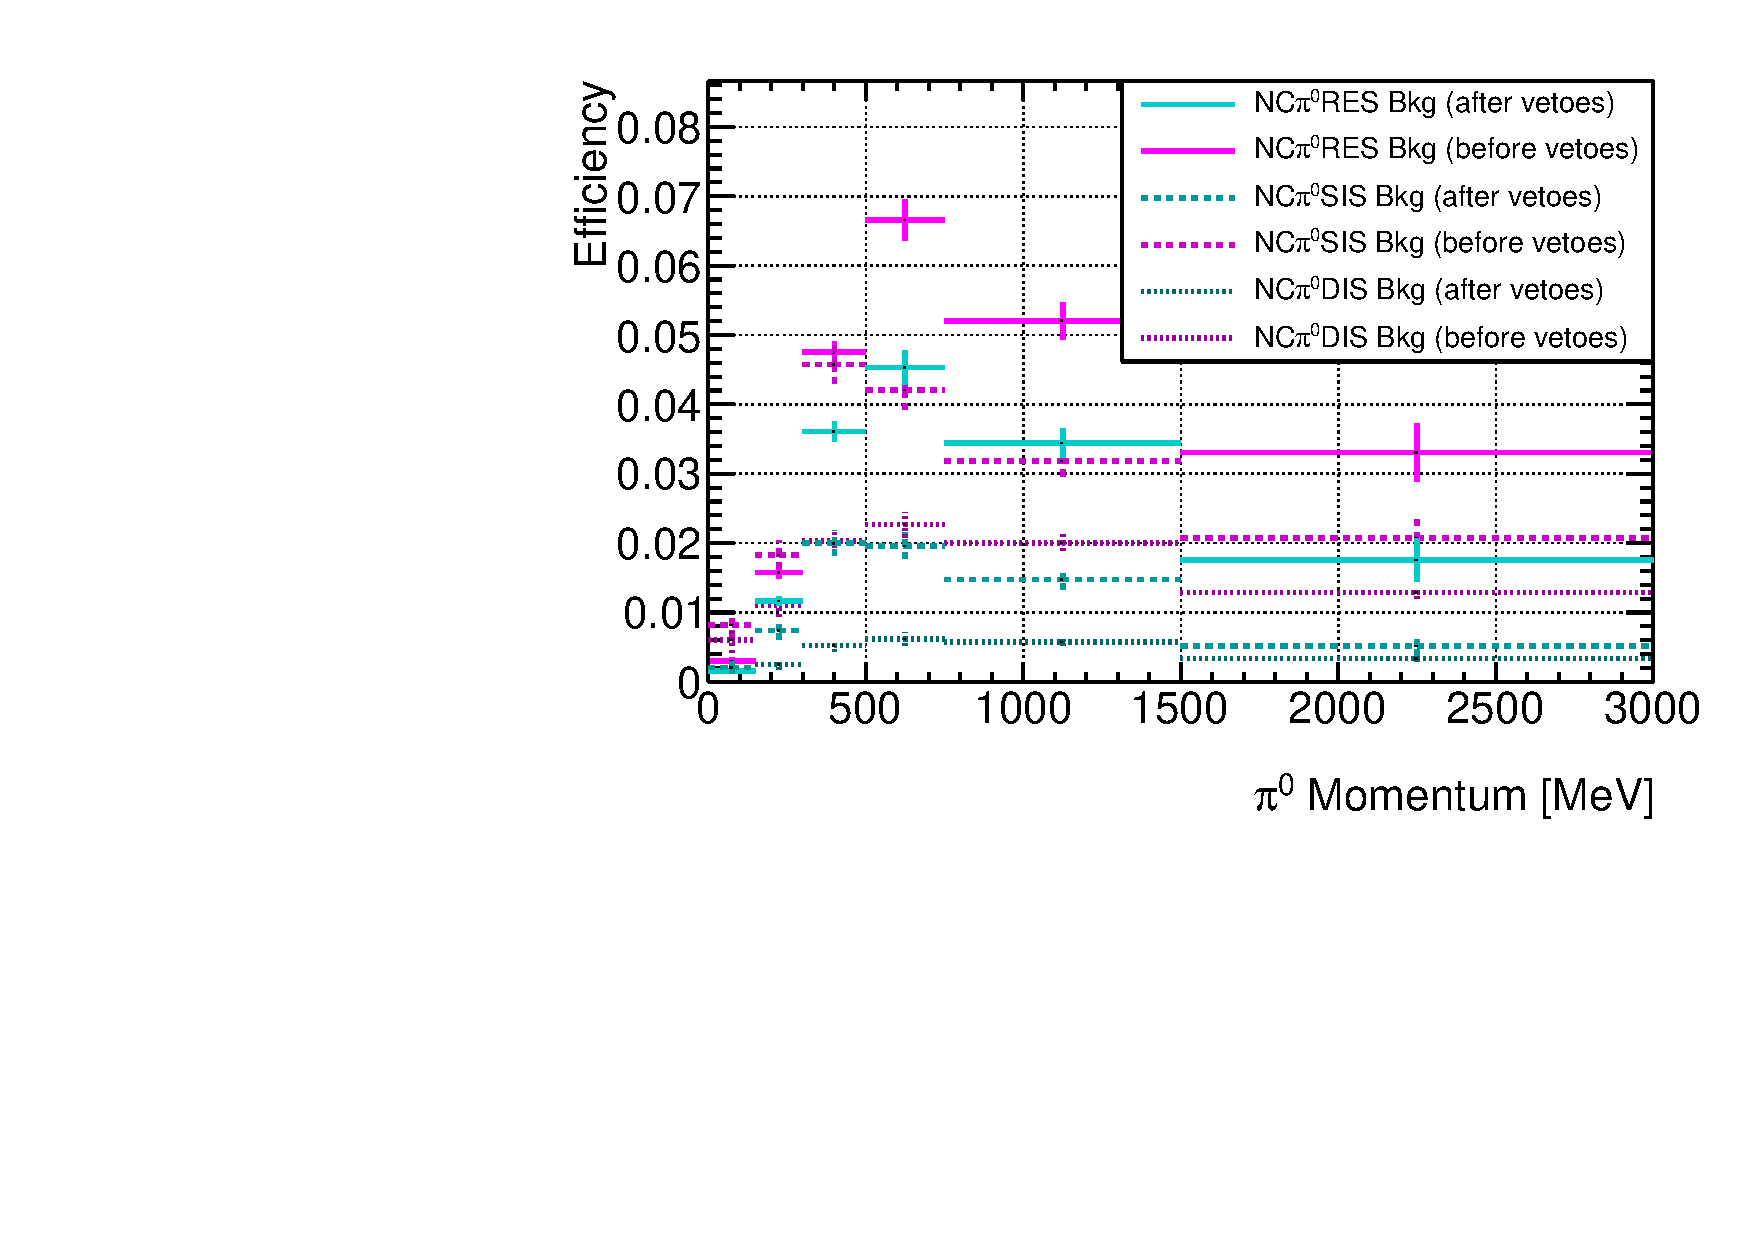
\includegraphics[width=0.8\textwidth]{images/NCg/Eff_1D_NCpPi0.pdf} \\
  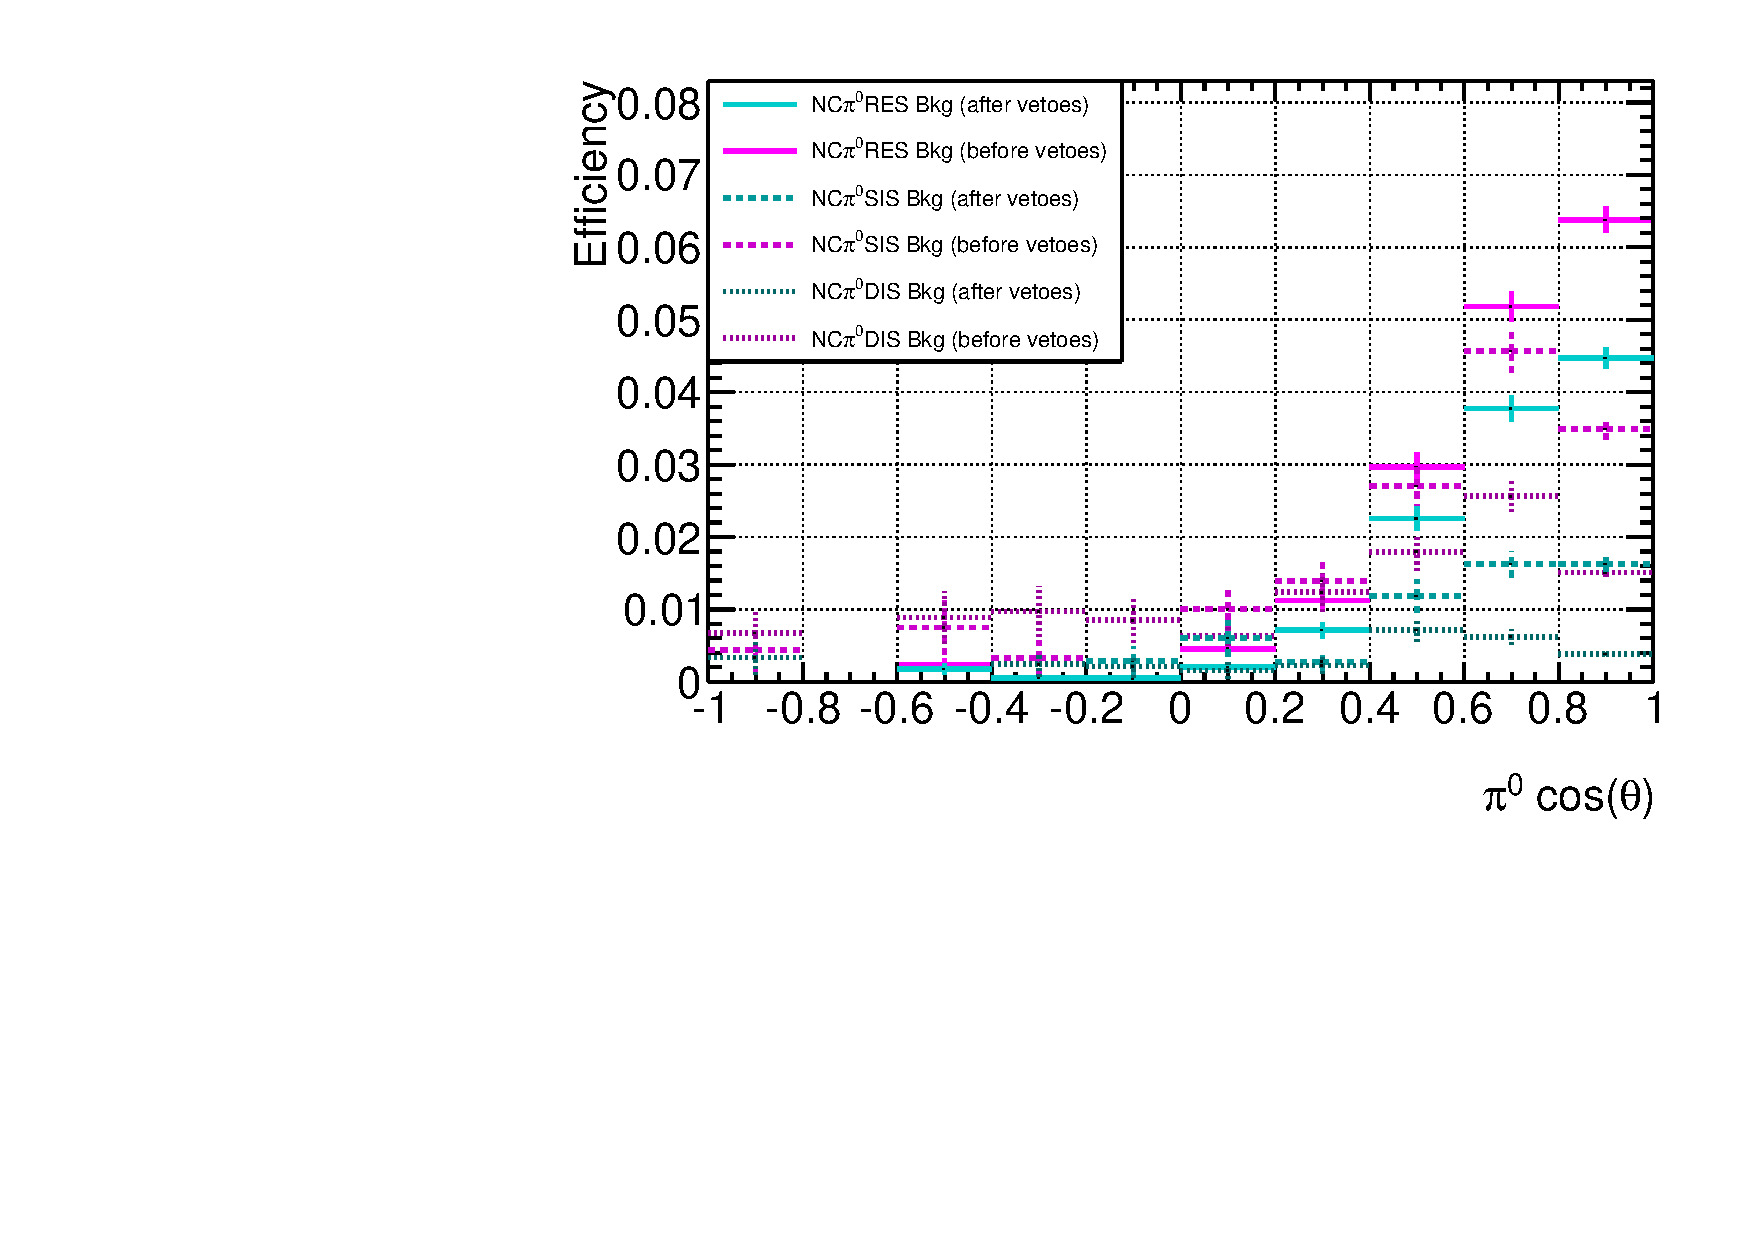
\includegraphics[width=0.8\textwidth]{images/NCg/Eff_1D_NCctPi0.pdf}
  \caption[Background selection efficiency for neutral pions before
  and after the vetoes]{Background selection efficiency for neutral
    pions before and after the vetoes (errors are
    statistical). \textbf{\textit{Top:}} Efficiency against the in
    pion momentum for \Gls{NC} interactions.
    \textbf{\textit{Bottom:}} Efficiency against the in pion angle for
    \Gls{NC} interactions. The signal definition is any neutral pion
    creating a photon in the \Gls{FGD}1.}
  \label{fig:pizeff1}
\end{figure}


\begin{figure}[ht]
  \center
  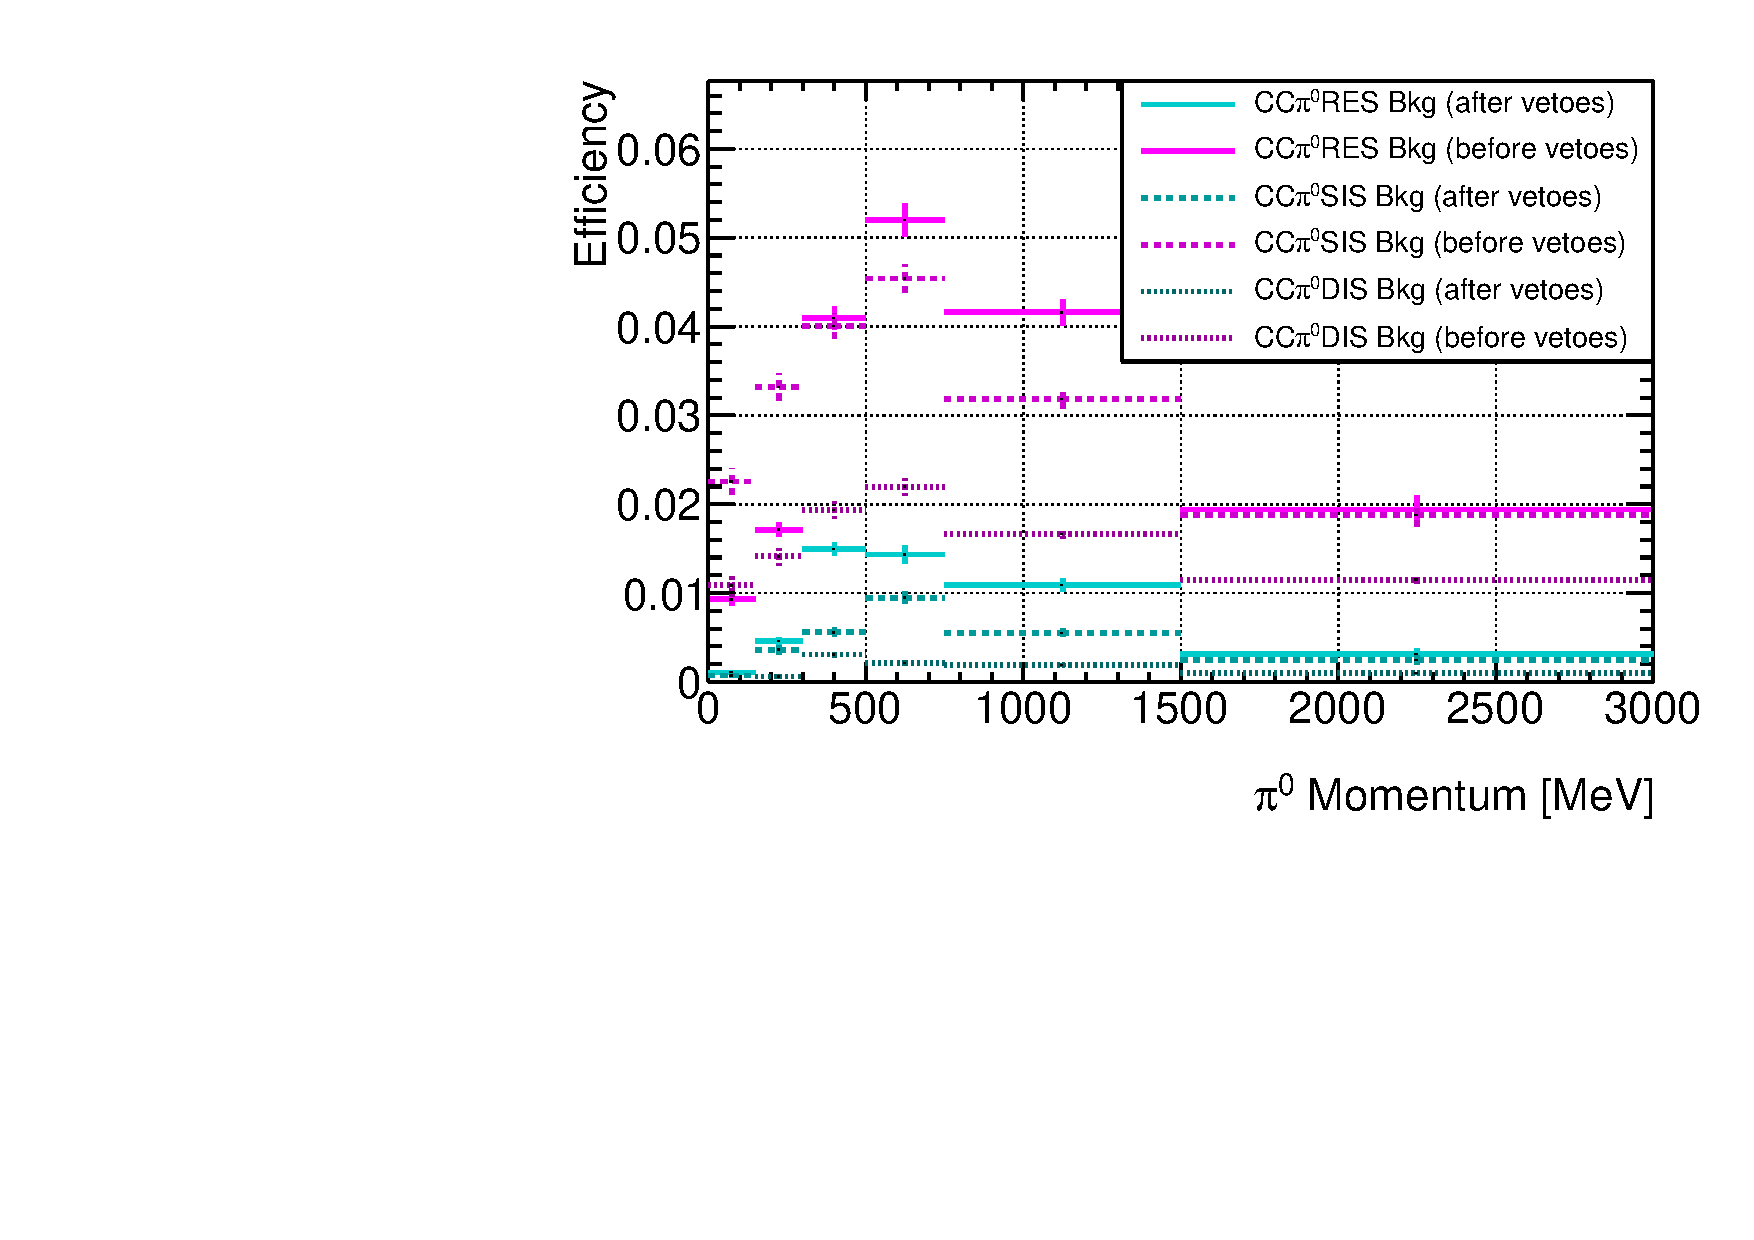
\includegraphics[width=0.8\textwidth]{images/NCg/Eff_1D_CCpPi0.pdf} \\
  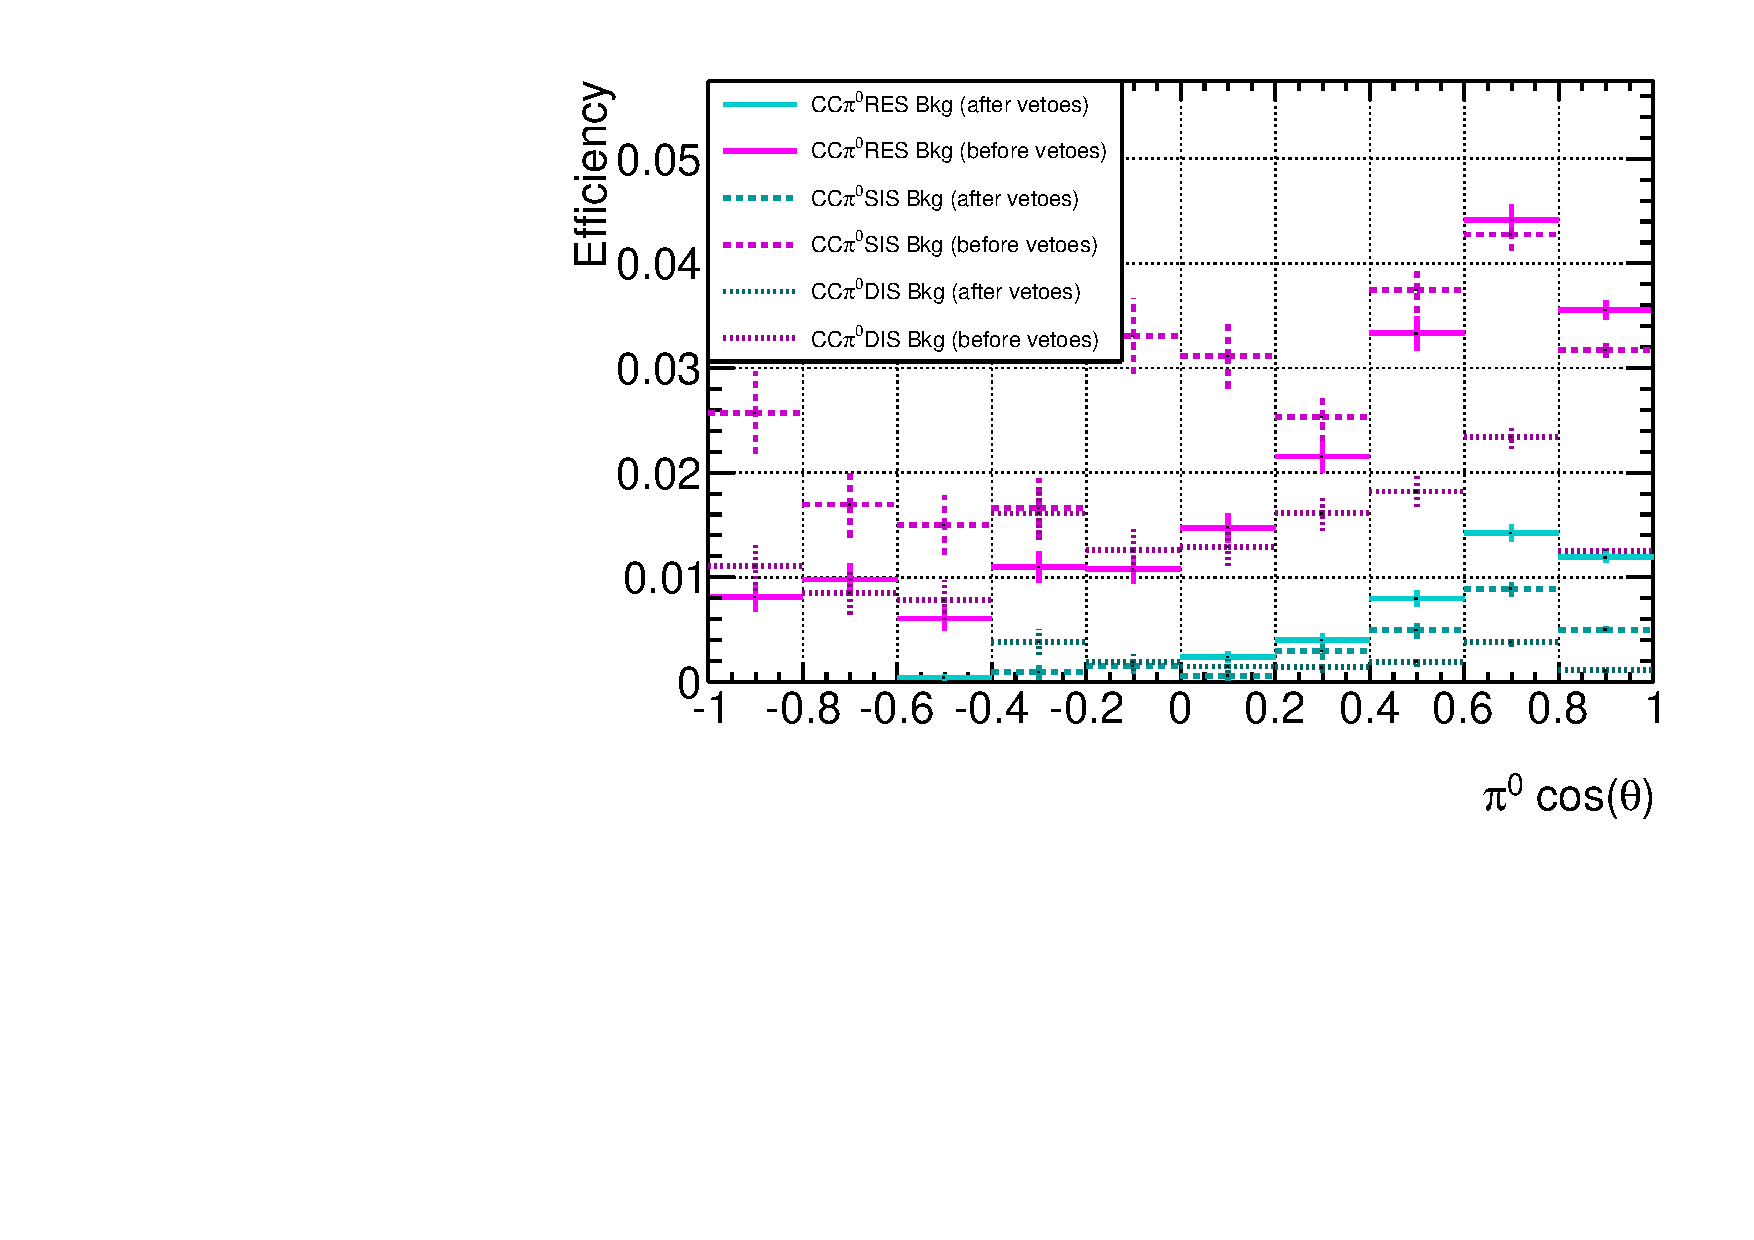
\includegraphics[width=0.8\textwidth]{images/NCg/Eff_1D_CCctPi0.pdf}
  \caption[Background selection efficiency for neutral pions before
  and after the vetoes]{Background selection efficiency for neutral
    pions before and after the vetoes (errors are
    statistical). \textbf{\textit{Top:}} Efficiency against the in
    pion momentum for \Gls{CC} interactions.
    \textbf{\textit{Bottom:}} Efficiency against the in pion angle for
    \Gls{CC} interactions. The signal definition is any neutral pion
    creating a photon in the \Gls{FGD}1.}
  \label{fig:pizeff2}
\end{figure}



%%% Local Variables:
%%% mode: latex
%%% TeX-master: "Thesis"
%%% End:
